\chapter{Fundamentação Teórica}

Neste capítulo são apresentados os conceitos relacionados ao desenvolvimento desta pesquisa, bem como o embasamento teórico necessário para o entendimento do estudo. Os temas abordados são: ETL, Banco de Dados NoSQL, Frameworks, Estudo Experimental de Software e trabalhos correlatos ao tema deste trabalho.


\clearpage
% ---

\section{ETL}

ETL sigla para \textit{Extraction, Transform and Load} (Extração, Limpeza/Transformação e Carga) é conhecido na literatura por definir processos que permitem a integração de dados, centralizando-os numa base destino facilitando o gerenciamento e análise dos dados [\cite{kimball:2004}]. O fluxo do processo de ETL inicia-se com extração dos dados a partir de uma fonte, que podem ser arquivos textuais, banco de dados relacionais ou banco de dados NoSQL. Os dados são propagados para uma Área de Processamento de Dados onde são executadas a limpeza e transformação por meio de mecanismos de ETL definidos como agregação, junção, filtro, união, entre outros. Finalmente, os dados são carregados em estruturas que podem ser data warehouses ou repositórios analíticos. 

\cite{kimball:2004} definem ETL em quatro macroprocessos, com 34 subsistemas. Os quadros \ref{subextracao}, \ref{sublimpeza}, \ref{subcarga} e \ref{subgerenciamento} mostram os subsistemas do processo de ETL. Os quatro macroprocessos são:

\begin{itemize}
	\item Extração: Recolhe os dados dos sistemas de origem e grava na área de processamento de dados antes de qualquer reestruturação significativa. Esta etapa possui 3 subsistemas.
	
	\item Limpeza e Transformação: Envia os dados de origem, por meio de várias etapas de processamento no sistema ETL. Melhora a qualidade dos dados recebidos da fonte, mescla dados de duas ou mais fontes para criar e aplica dimensões e métricas. Esta etapa possui 5 subsistemas.
	
	\item Entrega ou Carga: Estrutura fisicamente e carrega os dados conforme desejado em DWs ou repositórios analíticos. Esta etapa possui 13 subsistemas.
	
	\item Gerenciamento: Gerencia os sistemas e processos relacionados ao ambiente ETL de forma coerente. Esta etapa possui 13 subsistemas.
\end{itemize}
\clearpage

\begin{table}[h]
	\centering
	\caption{Subsistemas do macroprocesso de extração do processo de ETL}
	\label{subextracao}
	\begin{tabular}{|p{3cm}| p{11cm} |}
	\hline
	Macroprocesso & subsistema\\
	\hline
	Extração & \textbf{Data Profiling:} Explora uma origem de dados para determinar seu ajuste para inclusão como uma fonte associado à limpeza e ajuste de requisitos.\\
	&  \textbf{Change Data Capture:} Isola as mudanças ocorridas nos sistemas de origem, de forma a reduzir os processos de ETL - Carga Incremental.\\
	& \textbf{Sistema de Extração:} Extração e movimentação dos dados de origem para dentro do DW, para processamento futuro.\\
	\hline	
		
	\end{tabular}
\end{table}

\begin{table}[h]
	\centering
	\caption{Subsistemas do macroprocesso de limpeza e extração do processo de ETL}
	\label{sublimpeza}
	\begin{tabular}{|p{3cm}| p{11cm} |}
		\hline
		Macroprocesso & subsistema\\
		\hline
		Limpeza e Transformação &  \textbf{Data Cleasing System - Sistema de Limpeza de Dados:}  Implementa processos de qualidade de dados para identificar violações de qualidade.\\
		& \textbf{Error Event Tracking - Acompanhamento de erro:} Captura todos os ‘eventos de erro’, que serão as entradas vitais para a melhoria da qualidade dos dados.\\
		& \textbf{Criação de Dimensão de auditoria:} Junta Metadados para cada Tabela Fato, como uma dimensão. Este Metadados estará disponível para a geração de aplicações de BI que visualizem  a qualidade dos dados.\\
		& \textbf{Deduplication - Tirar a duplicidade de dados:} Elimina dados redundantes de dimensões, como clientes ou produtos. Pode requerer integração cruzada entre multiplas origens e a aplicação de regras para identificar qual a versão mais correta de uma linha duplicada.\\
		& \textbf{Data Conformance - conformidade de dados:} Força o uso de atributos comuns entre as principais Conformed Dimensions versus as métricas comuns nas Tabelas Fato relacionadas.\\
		\hline
		
	\end{tabular}
\end{table}

\clearpage


\begin{table}[h]
	\centering
	\caption{Subsistemas do macroprocesso de entrega ou carga do processo de ETL}
	\label{subcarga}
	\begin{tabular}{|p{3cm}| p{11cm} |}
		\hline
		Macroprocesso & subsistema\\
		\hline
		Entrega ou Carga & \textbf{Slowly Changing Dimension (SCD) Manager:} Implementa a lógica para os atributos SCD. \\
		& \textbf{Surrogate Key Generator:} Cria as chaves substitutas (chaves de negócio) - surrogate keys independentes para cada dimensão.  \\
		& \textbf{Hierarchy Manager:} Entrega multipla e simultânea de estruturas hierarquicas na dimensão. \\
		& \textbf{Special Dimensions Manager:} Cria locais - placeholders na estrutura de ETL para sustentar os processos repetitivos específicos da organização, no desenho de dimensões específicas coma as Junk Dimensions, Mini Dimensions e indicadores de comportamento. \\
		& \textbf{Fact Table Builders:} Construção dos três tipos básicos de tabela fato: Transacional, Periódico e Cumulativo (transaction grain, periodic snapshot e accumulating snapshot). \\
		& \textbf{Surrogate Key Pipeline:} Substitui, nas dimensões, a chave natural operacional das tabelas de origem pelas chaves substitutas (Surrogate Key) que serão utilizadas para o relacionamento com as tabelas fato.  \\
		& \textbf{Multi-Valued Bridge Table Builder:} Construção e Manutenção das tabelas ponte (bridge tables) para suportar os relacionamentos multi-valorados. \\
		& \textbf{Late Arriving Data Handler:} Aplica modificações especiais nas procedures do processo padrão para lidar com tabelas fato recém definidas (late-arriving)  e dimensões. \\
		& \textbf{Dimension Manager:} Centraliza a autoridade para preparar e divulgar as dimensões conforme (conformed dimensions) para a comunidade do Data Warehouse.  \\
		& \textbf{Fact Table Provider:} Detém a administração de uma ou mais tabelas fato, e a responsabilidade de criação, manutenção e uso. \\
		& \textbf{Aggregate Builder:} Construção e manutenção de agregações que serão usadas de forma continua com tecnologias de navegação agregada para melhorar a  performance das consultas.  \\
		& \textbf{OLAP Cube Builder:} Seleciona os dados do esquema dimensional para popular os cubos OLAP. \\
		& \textbf{Data Propagation Manager:} Prepara dados conformados e integrados no servidor de apresentação do Data Warehouse, para entrega em outros ambientes, para propósitos especiais. \\
		\hline
		
	\end{tabular}
\end{table}

\clearpage

\begin{table}[h]
	\centering
	\caption{Subsistemas do macroprocesso de gerenciamento do processo de ETL}
	\label{subgerenciamento}
	\begin{tabular}{|p{3cm}| p{11cm} |}
		\hline
		Macroprocesso & subsistema\\
		\hline
		Gerenciamento & \textbf{Job Scheduler:} A estratégia de gerenciamento da execução dos ETLs deve ser confiável, incluindo os relacionamentos e dependências entre os ETLs. \\
		& \textbf{Backup System:} Mantem cópia do ambiente de ETL para propósito de recuperação, restart e arquivamento. \\
		& \textbf{Recovery and Restart:} Processos para recuperação do ambiente de ETL  ou processo de reinicio, em caso de eventuais falhas. \\
		& \textbf{Version Control:} Mantem arquivadas versões dos ETLs, para eventual recuperação das lógicas e metadados do 'ETL pipeline'. \\
		& \textbf{Version Migration:} Migração de uma versão completa do 'ETL pipeline' a partir do ambiente de desenvolvimento para um ambiente de testes e, finalmente, para o ambiente de produção. \\
		& \textbf{Workflow Monitor:} Garante que os processos de ETL estão sendo eficientemente executados e que as cargas iniciem precisamente nas janelas de tempo estipuladas.  \\
		& \textbf{Sorting:} Garante a fundamental alta performance nos grupos de processos de ETLs. \\
		& \textbf{Lineage and Dependency:} Identifica a origem dos dados, as localizações intermediarias, as transformações e o dado final, permitindo acompanhar de forma estruturada, a trajetória dos dados até a sua carga no Data Warehouse. \\
		& \textbf{Problem Escalation:} Estrutura de suporte que  encaminha os problemas encontrados nos processos de  ETLs (erros)  para o nível de solução apropriado. \\
		& \textbf{Paralleling and Pipelining:} Habilita ao sistema de ETL a potencializar automaticamente  o uso de recursos como múltiplos processadores ou computação em grade (grid computing) para entregas dentro dos prazos restritos. \\
		& \textbf{Security:} Garante o acesso autorizado aos ETLs e Metadados, de forma individual ou em grupos, mantendo um histórico dos acessos.\\
		& \textbf{Compliance Manager:} Suporta os requerimentos organizacionais de conformidade, através, tipicamente, da manutenção da custódia da cadeia de dados e do acompanhamento dos acessos aos dados (quem teve o acesso autorizado ao dado). \\
		& \textbf{Metadata Repository:} Captura os metadados do ETL, incluindo os metadados de processo, metadados técnicos e metadados do negócio que significam todos os metadados do ambiente de DW/BI.\\
		\hline
		
	\end{tabular}
\end{table}

\clearpage


\section{Bancos de Dados NoSQL}

Consistem em bancos de dados não relacionais projetados para gerenciar grandes volumes de dados e que disponibilizam estruturas e interfaces de acesso simples (Lima; Mello, 2015). Cada SGBD (Sistema Gerenciador de Banco de Dados) NoSQL possui um esquema de modelagem diferente, nos quais são divididas pela literatura em quatro categorias amplamente usadas: Chave-Valor, Orientado a Documentos, Famílias de Colunas e Baseado em Grafos [\cite{fowler:2013}, \cite{kaur:2013}].

As principais características dos banco de dados NoSQL são: distribuído, escalabilidade horizontal, construído para grande volume de dados, BASE ao invés de ACID, modelo de dados não relacional, não suporta SQL [\cite{fowler:2013}, \cite{nasholm:2012}].

\subsection{Banco de dados Orientados à Documentos}

Banco de dados orientados a documentos são capazes de armazenar documentos como dado. Esses documentos podem ser em qualquer formato como XML (eXtensible Markup Language), YAML (Yet Another Markup Language), JSON (JavaScript Object Notation), entre outros. Os documentos são agrupados na forma de coleções. Comparando com banco de dados relacional, as coleções são como tabelas e os documentos como os registros. Porém, a diferença entre eles é que cada registro na tabela do banco relacional tem o mesmo número de campos, enquanto que na coleção do banco de dados orientado a documentos, podem ter campos completamente diferentes [\cite{kaur:2013}].

Existem mais de 15 banco de dados orientados a documentos disponíveis e os mais utilizados são MongoDB, CouchDB e o RavenDB [\cite{kaur:2013}].

\subsection{Banco de dados Famílias de Colunas}

Banco de dados baseados em Famílias de Colunas são desenvolvidos para abranger três áreas: número enorme de colunas, a natureza esparsa dos dados e frequentes mudanças no esquema. Os dados em Famílias de colunas são armazenados em colunas de forma contínua, enquanto que em bancos de dados relacionais as linhas é que são contínuas. Essa mudança faz com que operações como agregação, suporte para ad-hoc e consultas dinâmicas se tornem mais eficientes [\cite{kaur:2013}].

A maioria dos bancos de dados baseados em Famílias de Colunas são também compatíveis com o framework MapReduce, no qual acelera o processamento de enorme volume de dados pela distribuição do problema em um grande número de sistemas. Os bancos de dados  de Família de Colunas open-source mais populares são Hypertable, HBase e Cassandra [\cite{kaur:2013}].

\subsection{Banco de dados Baseado em Grafos}

Bancos de dados baseado em Grafos são como uma estrutura de rede contendo nós e arestas, onde as arestas interligam os nós representando a relação entre eles. Comparando com o modelo Entidade-Relacionamento, o nó corresponde à entidade, a propriedade do nó à um atributo, a relação entre as entidades ao relacionamento entre os nós. Nos bancos de dados relacionais as consultas requerem atributos de mais de uma tabela resultando numa operação de junção, por outro lado, bancos de dados baseado em Grafos são desenvolvidos para encontrar relações dentro de uma enorme quantidade de dados rapidamente, tendo em vista que não é preciso fazer junções, ao invés disso, ele fornece indexação livre de adjacência \cite{kaur:2013}.

\subsection{Banco de dados Chave-Valor}

Em Bancos de dados Chave-Valor os dados são organizados como uma associação de vetores de entrada consistindo em pares de chave-valor. Cada chave é única e é usada para recuperar os valores associados a ele. Esses bancos de dados podem ser visualizados como um banco de dados relacional contendo múltiplas linhas e apenas duas colunas: chave e valor. Buscas baseadas em chaves resultam num baixo tempo de execução, além disso, os valores podem ser qualquer coisa como objetos, hashes, entre outros [\cite{kaur:2013}].

Os bancos de dados Chave-Valor mais populares são Riak, Voldemort e Redis [\cite{kaur:2013}].


\section{Frameworks}

\textit{Frameworks} podem ser considerados aglomerados de softwares, onde estes são capazes de serem estendidos e adaptados para utilidades específicas [\cite{taligent:1994}]. \cite{pree:1997}, consideram que  \textit{frameworks} são aplicações semi-completas e que podem ser reutilizadas para especializar produtos de software customizados. \cite{sommerville:2013}, ressalta que \textit{framework} é uma estrutura genérica estendida com o intuito de criar uma aplicação mais específica e \cite{schmidt:2004} define como sendo um conjunto de artefatos de software (como classes, objetos e componentes) que colaboram para fornecer uma arquitetura reusável.

Os \textit{frameworks} possibilitam a reusabilidade de projeto, bem como ao reúso de classes específicas, pois fornecem uma arquitetura de esqueleto para a aplicação, que é definida por classes de objetos e suas interações. As classes são reusadas diretamente e podem ser estendidas usando-se recursos, como a herança \cite{sommerville:2013}. 

\cite{fayad:1997}, separam os \textit{frameworks} em três principais classes: de infraestrutura de sistema, de integração de \textit{middleware} e de aplicações corporativas. \textit{Frameworks} de infraestrutura de sistema apoiam o desenvolvimento de infraestruturas, como comunicações, interfaces de usuários e compiladores. Já os \textit{frameworks} de integração de \textit{middleware} são um conjunto de normas e classes de objetos associados que suportam componentes de comunicação e troca de informações. E finalmente, os \textit{frameworks} de aplicações corporativas estão relacionados com domínios de aplicação específicos, como sistemas financeiros. Eles incorporam conhecimentos sobre o domínios de aplicações e apoiam o desenvolvimento para o usuário final.

Muitas vezes, os \textit{frameworks} são implementações de padrões de projeto, como por exemplo o \textit{framework} MVC (Model-View-Control). A natureza geral dos padrões e o uso de classes abstratas e concretas permitem a extensibilidade \cite{sommerville:2013}.

Para estender um \textit{framework} não é necessário alterar o seu código, apenas é preciso adicionar classes concretas que herdam operações de classes abstratas. Ademais, há a possibilidade de definir \textit{callbacks}, que são métodos chamados em resposta a eventos reconhecidos pelo \textit{framework}.Esses métodos são reconhecido como 'inversão de controle' (\cite{schmidt:2004}). A figura \ref{inversaodecontrole} expressa o funcionalidade da inversão de controle. Os responsáveis pelo controle no sistema são os objetos do \textit{framework}, ao invés de serem objetos específicos de aplicação. E em resposta aos eventos de interface do usuário, banco de dados, entre outros, esses objetos do \textit{framework} invocam 'métodos hook' que, em seguida, são vinculados à funcionalidade fornecida ao usuário. A funcionalidade específica de aplicação responde ao evento de forma adequada. Por exemplo, um \textit{framework} terá um método que lida com um toque em uma tecla a partir do ambiente. Esse método chama o método \textit{hook}, que deve ser configurado para chamar os métodos de aplicação adequada para tratar o toque na tecla (\cite{sommerville:2013}).

\begin{figure}[h!]
	\centering
	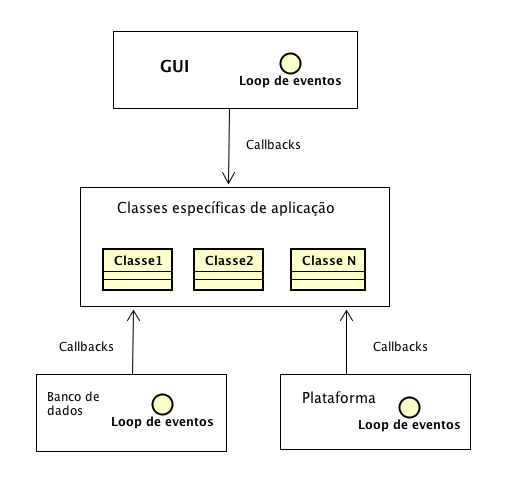
\includegraphics[scale=0.5]{fig/inversaodecontrole.png}
	\caption{Inversão de controle em \textit{framework}. (Adaptado de \cite{sommerville:2013})}
	\label{inversaodecontrole}
\end{figure}

O \textit{framework} ETL4NoSQL encaixa-se na categoria de aplicações corporativas, pois serve como base para aplicações de ETL, incorporando conhecimentos sobre a área de domínio para apoiar o desenvolvimento ao usuário final.




\section{Estudo Experimental de Software}

Segundo Travassos (2002), a experimentação é o centro do processo científico, por meio dos experimentos que é possível verificar teorias, explorar fatores críticos e formular novas teorias. O autor reforça ainda a necessidade de avaliar novas invenções e sugestões em comparação com as existentes.

Para Wohlin00, existem quatro métodos relevantes para experimentação em Engenharia de Software: científico, de engenharia, experimental e analítico. 

O paradigma indutivo, ou método científico, observa o mundo, pode ser utilizado quando se quer entender o processo, produto de software, ambiente. Ele mede e analisa, verifica as hipóteses do modelo ou teoria.  Já o método de engenharia observa as soluções existentes, é uma abordagem baseada na melhoria evolutiva, modifica modelos de processos ou produtos de softwares existentes com propósito de melhorar os objetos de estudo. O método experimental é uma abordagem baseada na melhoria revolucionária. Ela sugere um modelo, não necessariamente baseado em um existente, aplica o método qualitativo e/ou quantitativo, faz a experimentação, analisa e repete o processo. Por fim, o método analítico sugere uma teoria formal, é um método dedutivo que oferece uma base analítica para o desenvolvimento de modelos (Travassos, 2002).

Travassos (2002) sugere que a abordagem mais apropriada para a experimentação na área de Engenharia de Software seja o método experimental, pois considera a proposição e avaliação do modelo com os estudos experimentais.

Os principais objetivos relacionados à execução de um estudo experimental de software são: caracterização, avaliação, previsão, controle e melhoria a respeito de produtos, processos, recursos, modelos e teorias.

Os elementos principais do experimento são: as variáveis, os objetos, os participantes, o contexto do experimento, hipóteses e o tipo de projeto do experimento.

Esta pesquisa de dissertação considera a execução do estudo experimental de software para caracterizar, avaliar e propor melhorias ao framework ETL4NoSQL. O objetivo principal da aplicação do experimento é definir se o framework proposto é uma ferramenta adequada para auxiliar no desenvolvimento de processos de ETL em dados estruturados, semi estruturados e não estruturados. Os participantes escolhidos foram as principais ferramentas de ETL encontradas na literatura. Os questionários utilizados para a coleta de dados são baseadas nos requisitos mínimos considerados pela literatura para ferramentas de ETL.


\section{Trabalhos Correlatos}
Esta seção aborda os trabalhos que são correlatos a esta pesquisa, bem como descreve como estes trabalhos diferem do realizado
por esta pesquisa.

ARKTOS II: modela os processos de ETL

ETLMR: lida com os processos de ETL utilizando MapReduce

PygramETL: 

CloudETL:

P-ETL:

Big-ETL: Foca na paralelização e distribuição.

FramETL

Pentaho

Talend Studio for Data Integration

CloverETL

Oracle Data Integrator (ODI)